\documentclass[sigconf]{acmart}

\usepackage{graphicx}
\usepackage{pgfplots}

\usepackage{amssymb}
\usepackage{amsmath}
\usepackage{booktabs}

\usepackage{enumitem}
\usepackage{marginnote}
\setlength{\marginparwidth}{15mm}
\setlength{\marginparsep}{1mm}
\definecolor{darkblue}{rgb}{0.0,0.0,0.3}
\newcommand\todo[1]{\textcolor{blue}{[TODO: #1]}}
\newcommand\TODO[1]{\textcolor{blue}{\small [#1]}}
\newcommand\TODOM[1]{\marginpar{\color{blue}\renewcommand{\baselinestretch}{0.8}\tiny\tolerance=100000\hyphenpenalty=0\raggedright #1}}

% Input Graph

\def\iG{G}  % Input graph
\def\iV{V}  % Input nodes
\def\iv{v}  % Input node
\def\iE{E}  % Input edges
\def\ie{e}  % Input edge

% Drawing

\newcommand\drawing[1]{\mathcal{D}_{#1}}  % Drawing of graph
\newcommand\initdrawing[1]{\drawing{#1}^*}  % Drawing of graph

\def\drawingcurvesym{c}  % edge curve part of drawing
\def\drawingpossym{p}    % node position part of drawing

\newcommand\drawingcurve[1]{\drawingcurvesym(#1)}  % Drawing curve of argument edge
\newcommand\drawingpos[1]{\drawingpossym(#1)}  % Drawing pos urve of argument node

% Grid

\def\gScale{C}
\def\gmind{\hat d}


% Octilinear grid graph

\def\gG{\Gamma}  % Grid graph
\def\gV{\Psi}  % Grid graph nodes
\def\gv{\psi}  % Grid graph node
\def\gE{\Omega}  % v edges
\def\ge{\omega}  % Grid graph edge

\newcommand\ggv[2]{\gv_{#1, #2}}  % Grid node at #1, #2
\newcommand\gpv[3]{\gv_{#1, #2}^{#3}}  % Port #3 node at #1, #2
\newcommand\gse[3]{\ge_{#1, #2}^{#3}}  % Sink edge #3 node at #1, #2
\newcommand\gbe[4]{\ge_{#1, #2}^{#3, #4}}  % Bend edge for angle #4 at port #3 at node at #1, #2

\def\gPath{p}    % path on grid graph
\def\gPathOcti{p'}    % path on octilinear grid graph

\newcommand\gPturn[1]{c_{#1}}  % Turn penalty
\newcommand\gPturnEdge[1]{c'_{#1}}  % Turn penalty
\def\gHopcost{c_h}    % Hop cost in grid graph
\def\gHopcostOcti{c'_h}    % Hop cost in grid graph
\def\gSinkcost{c_s}    % Hop cost in grid graph
\newcommand\gPcost[1]{c(#1)}  % Path cost
\newcommand\gPcostOcti[1]{c'(#1)}  % Octilinear path cost

% ILP

\newcommand\gvused[2]{x_{#1#2}}	% bin. decision variable whether grid node #1 is assigned to input node #2
\newcommand\geused[2]{x_{#1#2}}	% bin. decision variable whether grid edge #1 is used be input edge #2

\newcommand\dir[2]{\delta_{#1#2}}	% variable telling the direction of edge #2 at node #1
\newcommand\dirdiff[2]{\Delta_{#1#2}}	% variable telling the direction difference of edge #1 and edge #2

\newcommand\bend[3]{\Delta_{#1#2}^{#3}}	% variable telling the direction difference of edge #1 and edge #2

\def\ldeg{\text{ldeg}}

\usepackage{tikz}
\usetikzlibrary{calc,trees,positioning,arrows,chains,shapes.geometric,%
  decorations.pathreplacing,decorations.pathmorphing,shapes,%
  matrix,shapes.symbols,plotmarks,decorations.markings,shadows}

\DeclareMathOperator{\atantwo}{atan2}

% Copyright
%\setcopyright{none}
%\setcopyright{acmcopyright}
%\setcopyright{acmlicensed}
\setcopyright{rightsretained}
%\setcopyright{usgov}
%\setcopyright{usgovmixed}
%\setcopyright{cagov}
%\setcopyright{cagovmixed}

% DOI
%\acmDOI{10.475/123_4}

% ISBN
%\acmISBN{123-4567-24-567/08/06}

%Conference
\acmConference[SIGSPATIAL '20]{SIGSPATIAL '20}{November 3-6 2020}{Seattle, Washington, USA}
\acmYear{2020}
\copyrightyear{2020}

\renewcommand{\topfraction}{0.96}
\renewcommand{\textfraction}{0.01}
\renewcommand{\floatpagefraction}{0.96}

\def\Hms{\makebox[1.6mm][l]{\hspace{0.2mm}\footnotesize ms}}
\def\Hs{\makebox[1.6mm][l]{\hspace{0.2mm}\footnotesize s}}
\def\Hk{\makebox[1.6mm][l]{\hspace{0.2mm}\footnotesize k}}
\def\Hm{\makebox[1.6mm][l]{\hspace{0.2mm}\footnotesize m}}
\def\Hh{\makebox[1.6mm][l]{\hspace{0.2mm}\footnotesize h}}
\def\Hhline{\\[.7mm]\hline}

\makeatletter
\DeclareRobustCommand*\cal{\@fontswitch\relax\mathcal}
\makeatother

\DeclareMathOperator*{\argmin}{\arg\!\min}
\DeclareMathOperator*{\argmax}{\arg\!\max}
\DeclareMathOperator*{\TED}{TED}
\DeclareMathOperator*{\lev}{lev}

\begin{document}
\title{Fast Generation of Metro Maps on Variable Base Grids}

\author{Hannah Bast}
\affiliation{%
  \institution{University of Freiburg}
  \city{Freiburg}
  \state{Germany}
}
\email{bast@cs.uni-freiburg.de}

\author{Patrick Brosi}
\affiliation{%
  \institution{University of Freiburg}
  \city{Freiburg}
  \state{Germany}
}
\email{brosi@cs.uni-freiburg.de}

\author{Sabine Storandt}
\affiliation{%
  \institution{University of Konstanz}
  \city{Konstanz}
  \state{Germany}
}
\email{sabine.storandt@uni-konstanz.de}

\begin{abstract}
Our interest is threefold. First, we would like to speed up the solution times of both the Linear Program and the approximation algorithm by using more sparse base grids. Second, we are interested in the capability of the original approach to render maps which are not octilinear, but for example orthoradial. Last, we want to investigate how a different base grid can be used to enlarge areas of high station density. 
\end{abstract}

%
% The code below should be generated by the tool at
% http://dl.acm.org/ccs.cfm
% Please copy and paste the code instead of the example below.
%
\begin{CCSXML}
<ccs2012>
<concept>
<concept_id>10002951.10003227.10003236.10003237</concept_id>
<concept_desc>Information systems~Geographic information systems</concept_desc>
<concept_significance>500</concept_significance>
</concept>
<concept>
<concept_id>10003752.10003809.10003636.10003811</concept_id>
<concept_desc>Theory of computation~Routing and network design problems</concept_desc>
<concept_significance>500</concept_significance>
</concept>
</ccs2012>
\end{CCSXML}

\ccsdesc[500]{Information systems~Geographic information systems}
\ccsdesc[500]{Theory of computation~Routing and network design problems}

\keywords{Public Transit, Map Matching, Schedule Data, GTFS}

\maketitle

\section{Introduction}

\begin{figure}
    \centering
	\vspace{-0.6cm}
	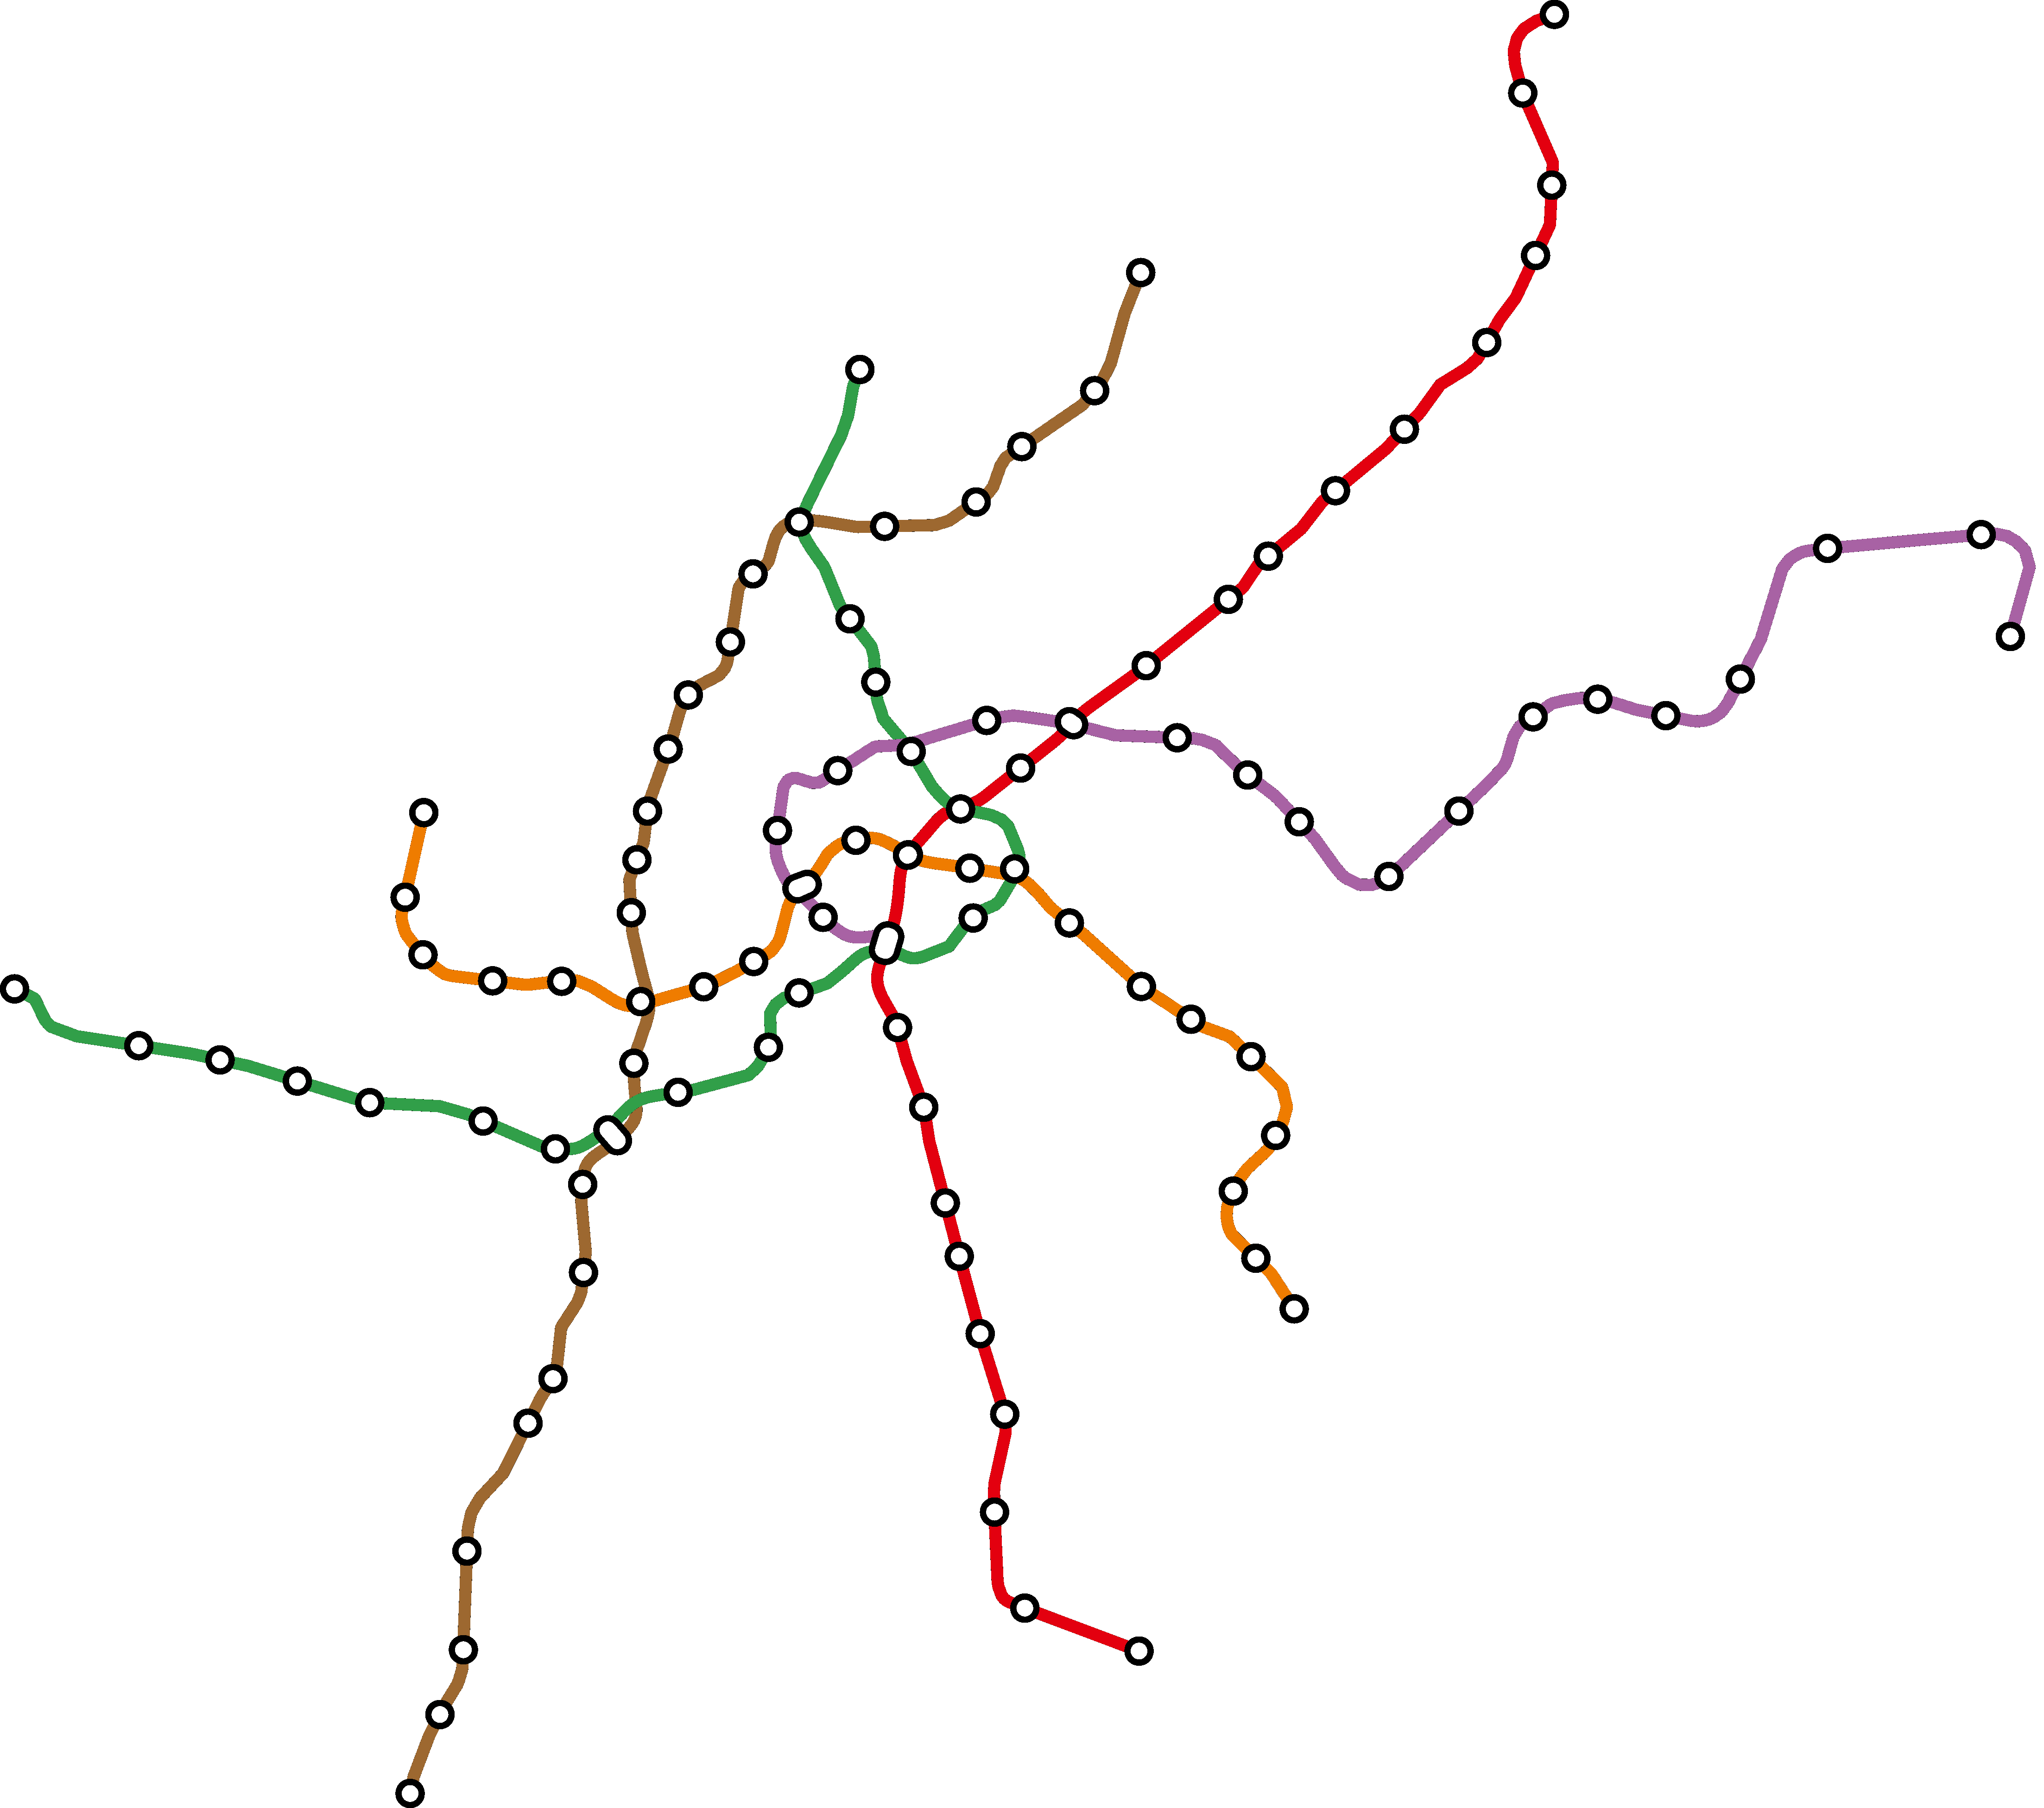
\includegraphics[width=0.27\textwidth]{figures/octi_input.pdf}
	\hspace{-1.3cm}
	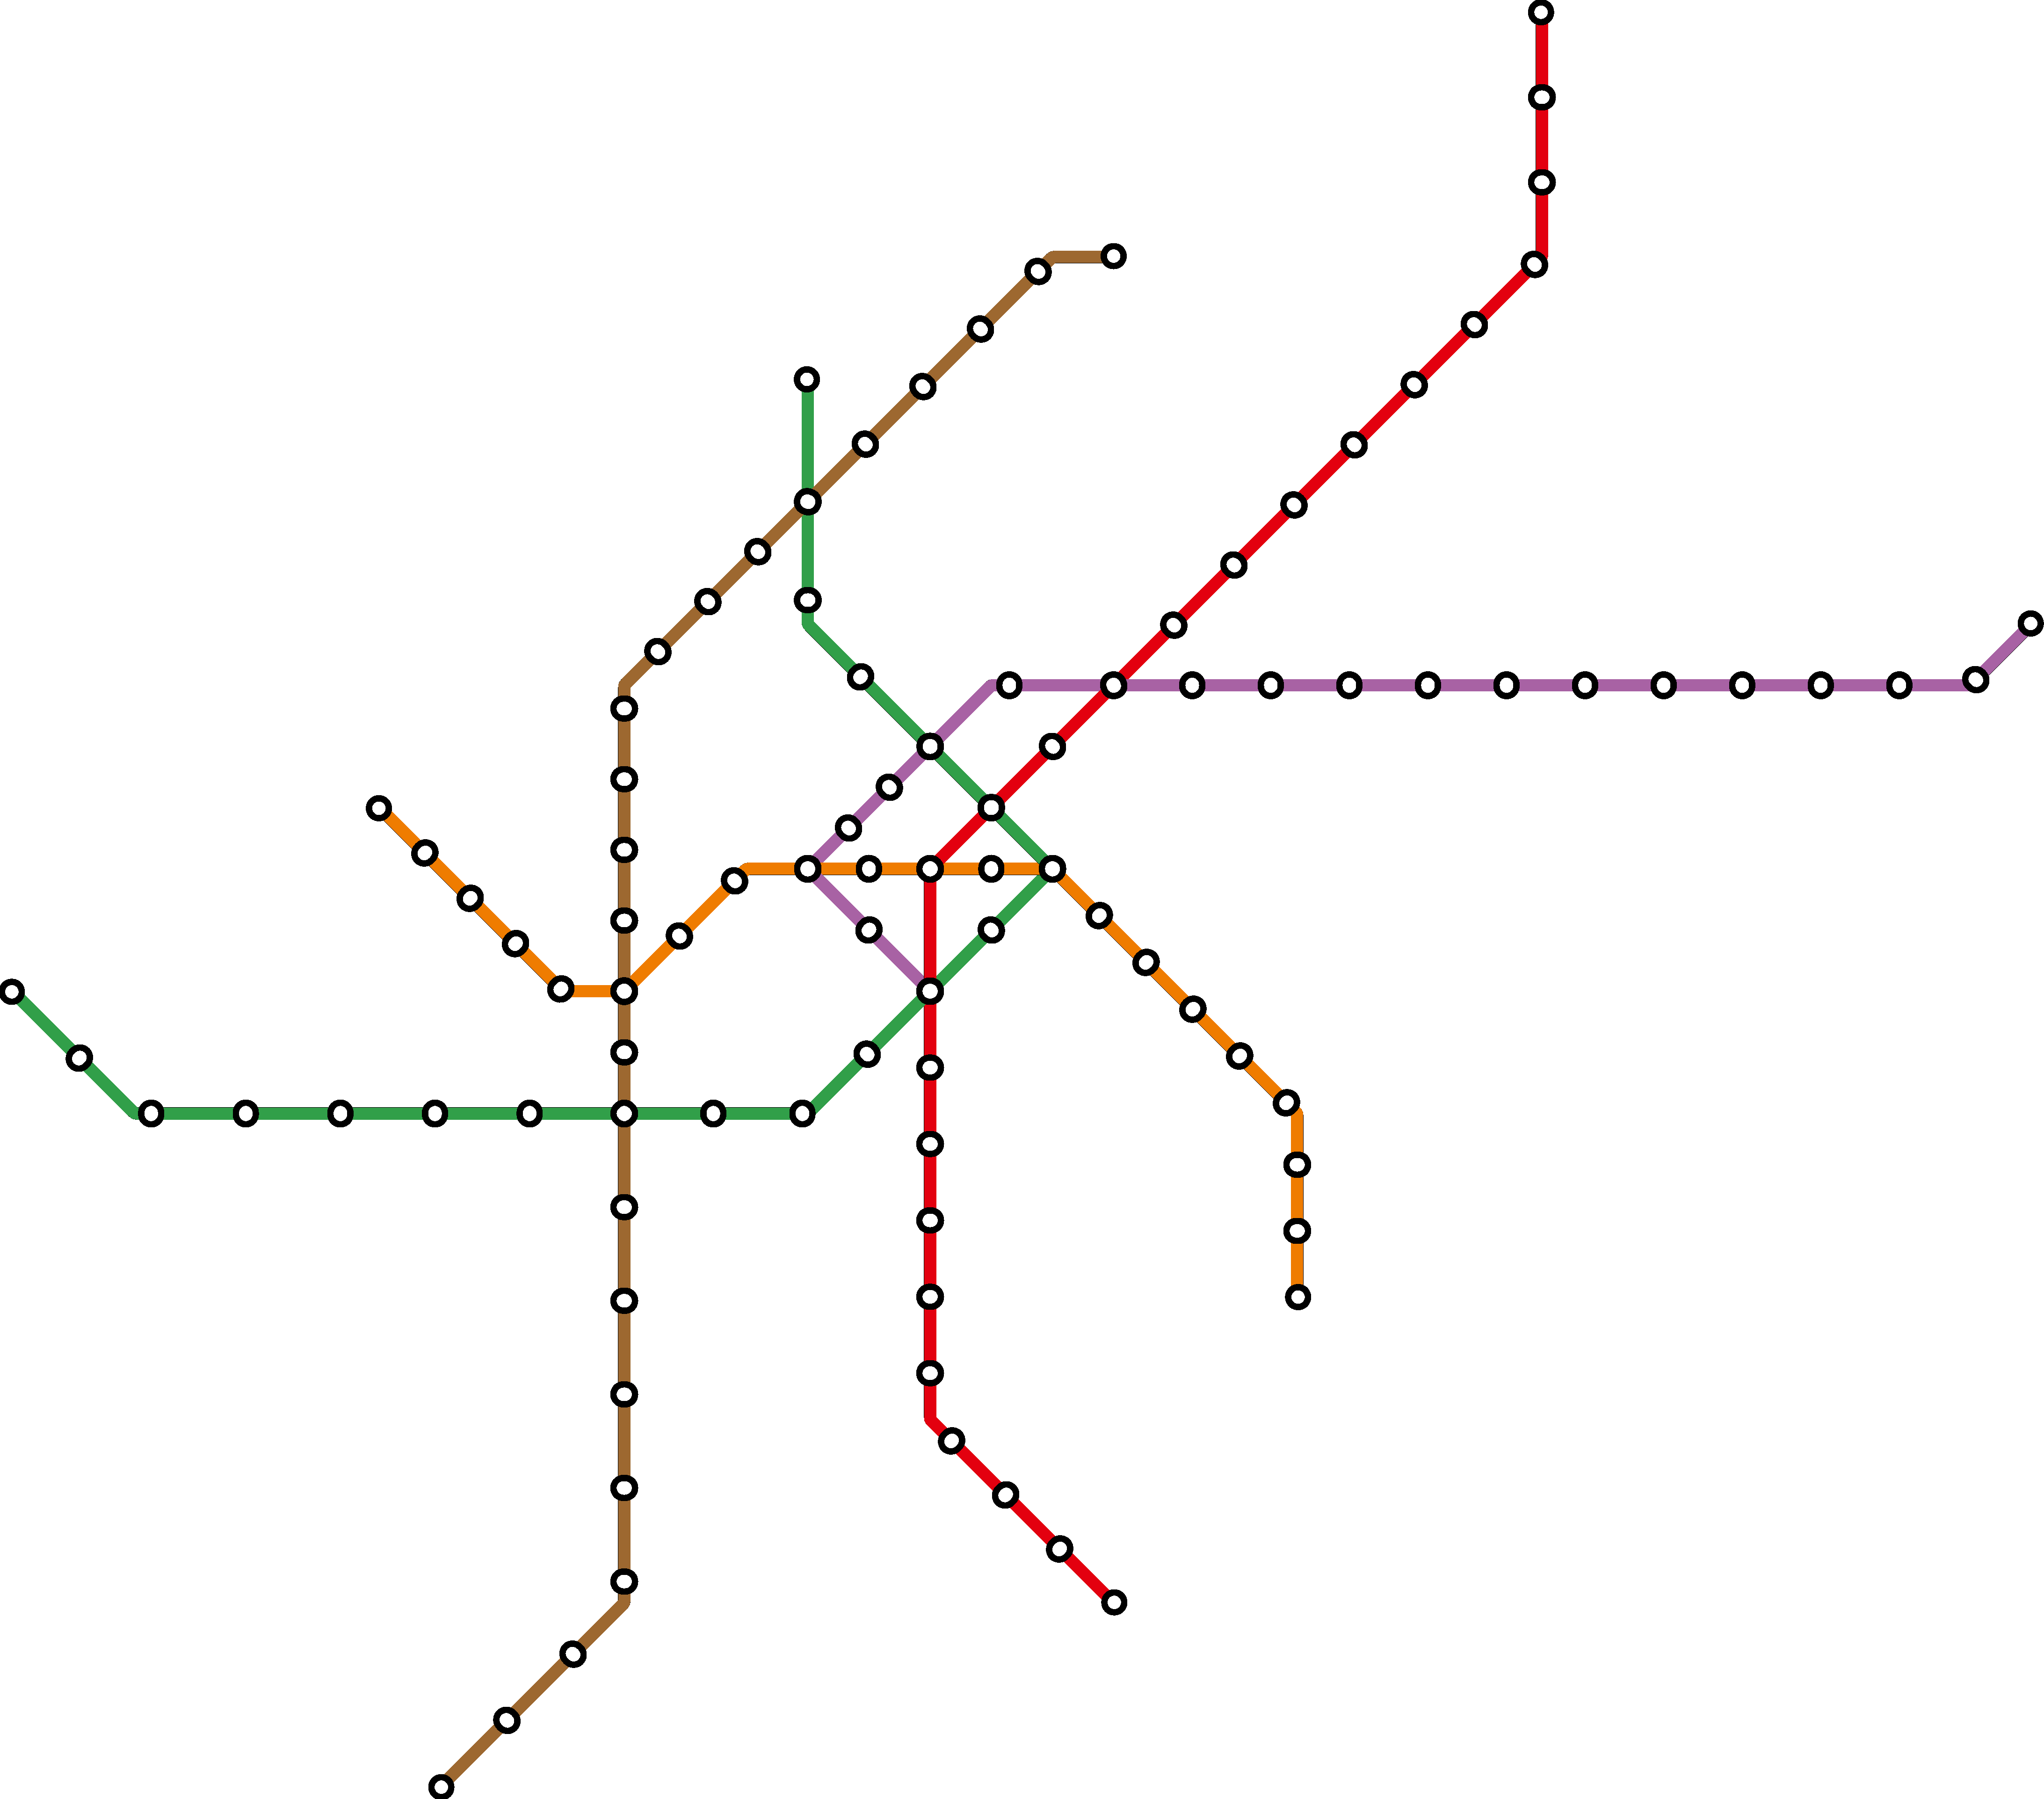
\includegraphics[width=0.27\textwidth]{figures/octi.pdf}
	\vspace{-.5cm}
	\caption{Left: The Vienna subway network, drawn with real-world geographical station positions and line courses. Right: Octilinear drawing by our approx. approach. Octilinearization took 202 ms.}
	\label{FIG:wien}
	\vspace{-.65cm}
\end{figure}

\subsection{Contributions}
\label{SEC:contrib}
%
We consider the following as our main contributions:
\begin{itemize}[parsep=0.5mm,leftmargin=0mm,itemindent=4mm]
\item A
\item B
\end{itemize}

\subsection{Problem definition}
\label{SEC:def}

\subsection{Related Work}
\label{SEC:related}

\begin{figure}
    \centering
	\hfill
	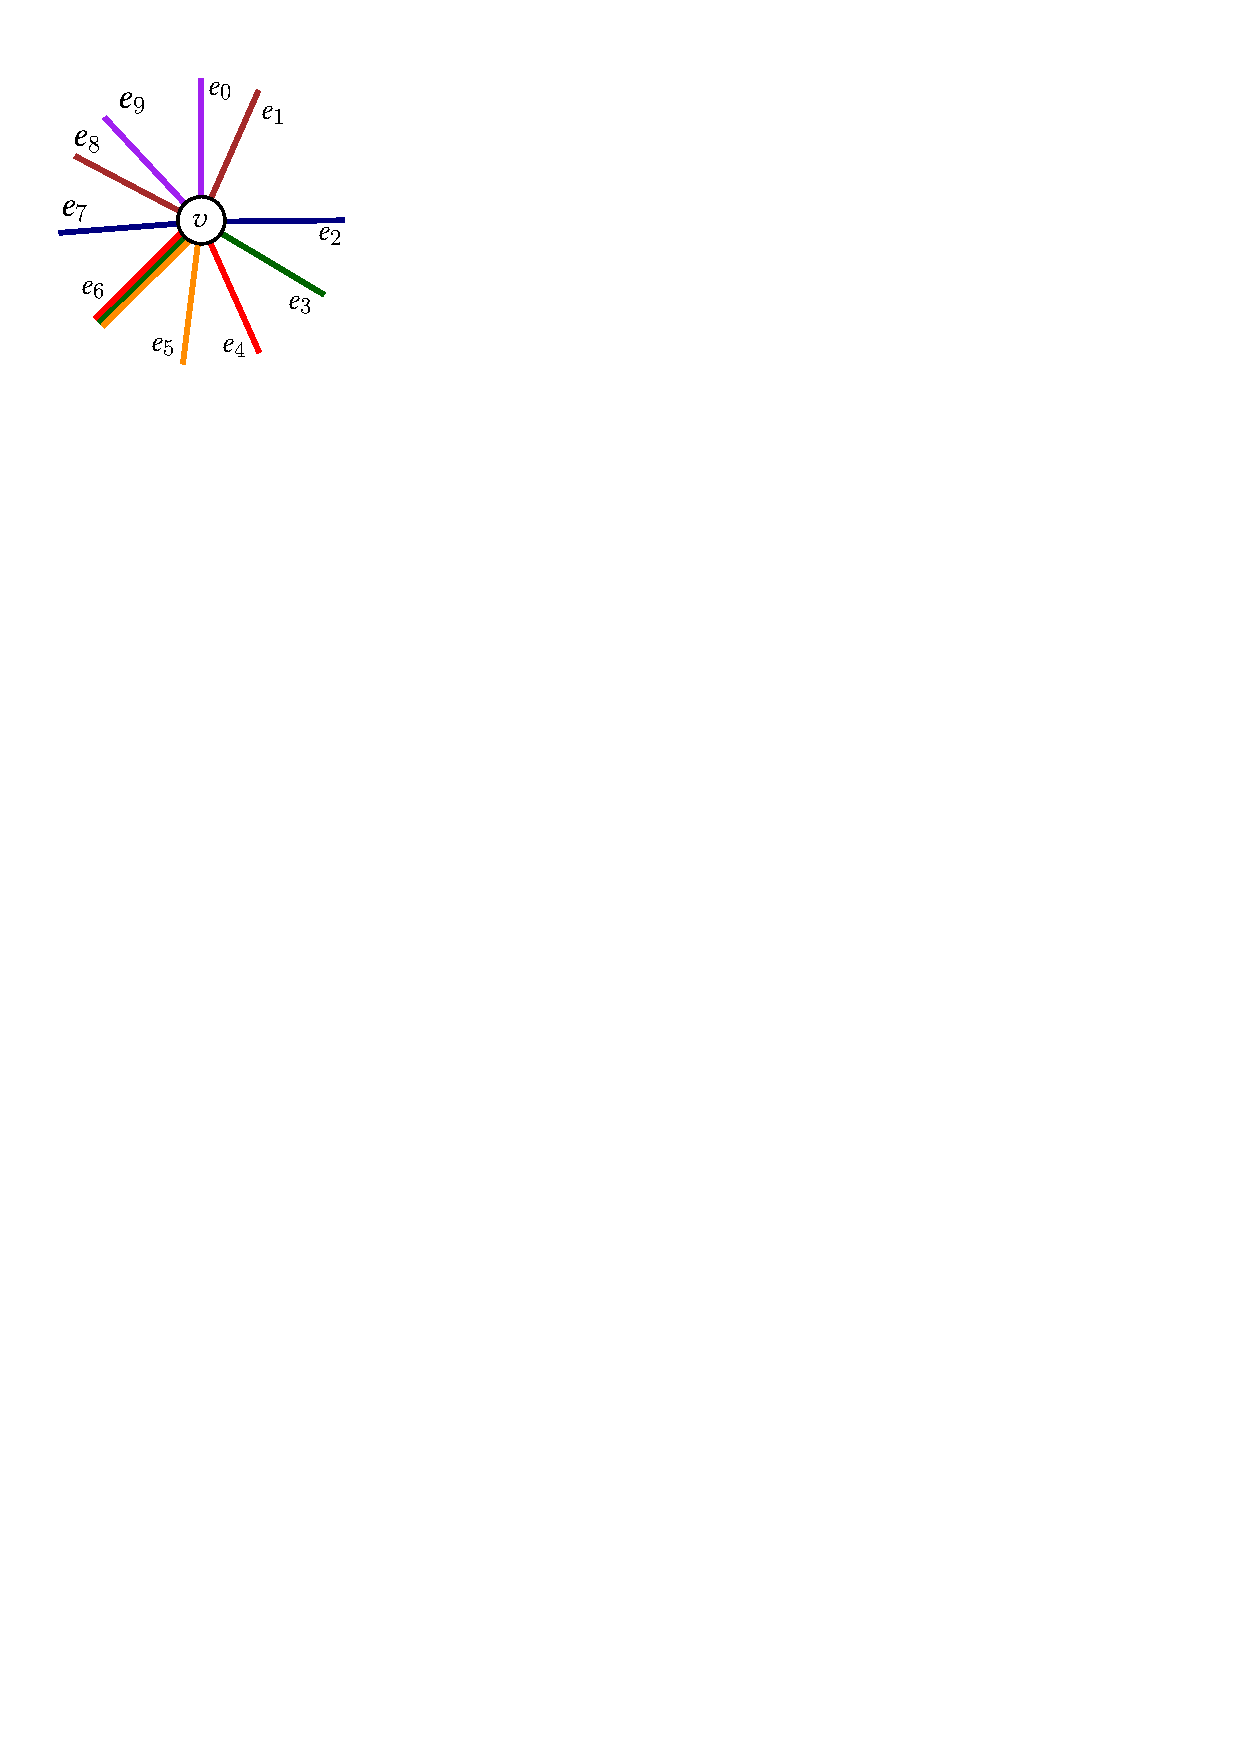
\includegraphics[width=0.18\textwidth]{figures2/nodesplit.pdf}
	\hfill
	\includegraphics[width=0.18\textwidth,page=2]{figures2/nodesplit.pdf}
	\hfill
	\caption{Left: Node $v$ in an input line graph has a degree of 10, making it impossible to render the graph in an octilinear fashion. Right: We keep the first (in clockwise order) 7 adjacent edges of $v$, combine the lines of the remaining edges $e_7$, $e_8$ and $e_9$ into a single new edge $e'_0$ and connect it to a new non-station node $v'$. In reality, $v'$ is given the exact same location as $v$ to not distort node move penalties later on.}
	\label{FIG:orthoradgrid}
\end{figure}

\section{Node Splitting}


\section{Octilinear Hanan Grid}

\section{Quad-Tree Grid}

\section{Ortho-Radial Grid}

\begin{figure}
    \centering
	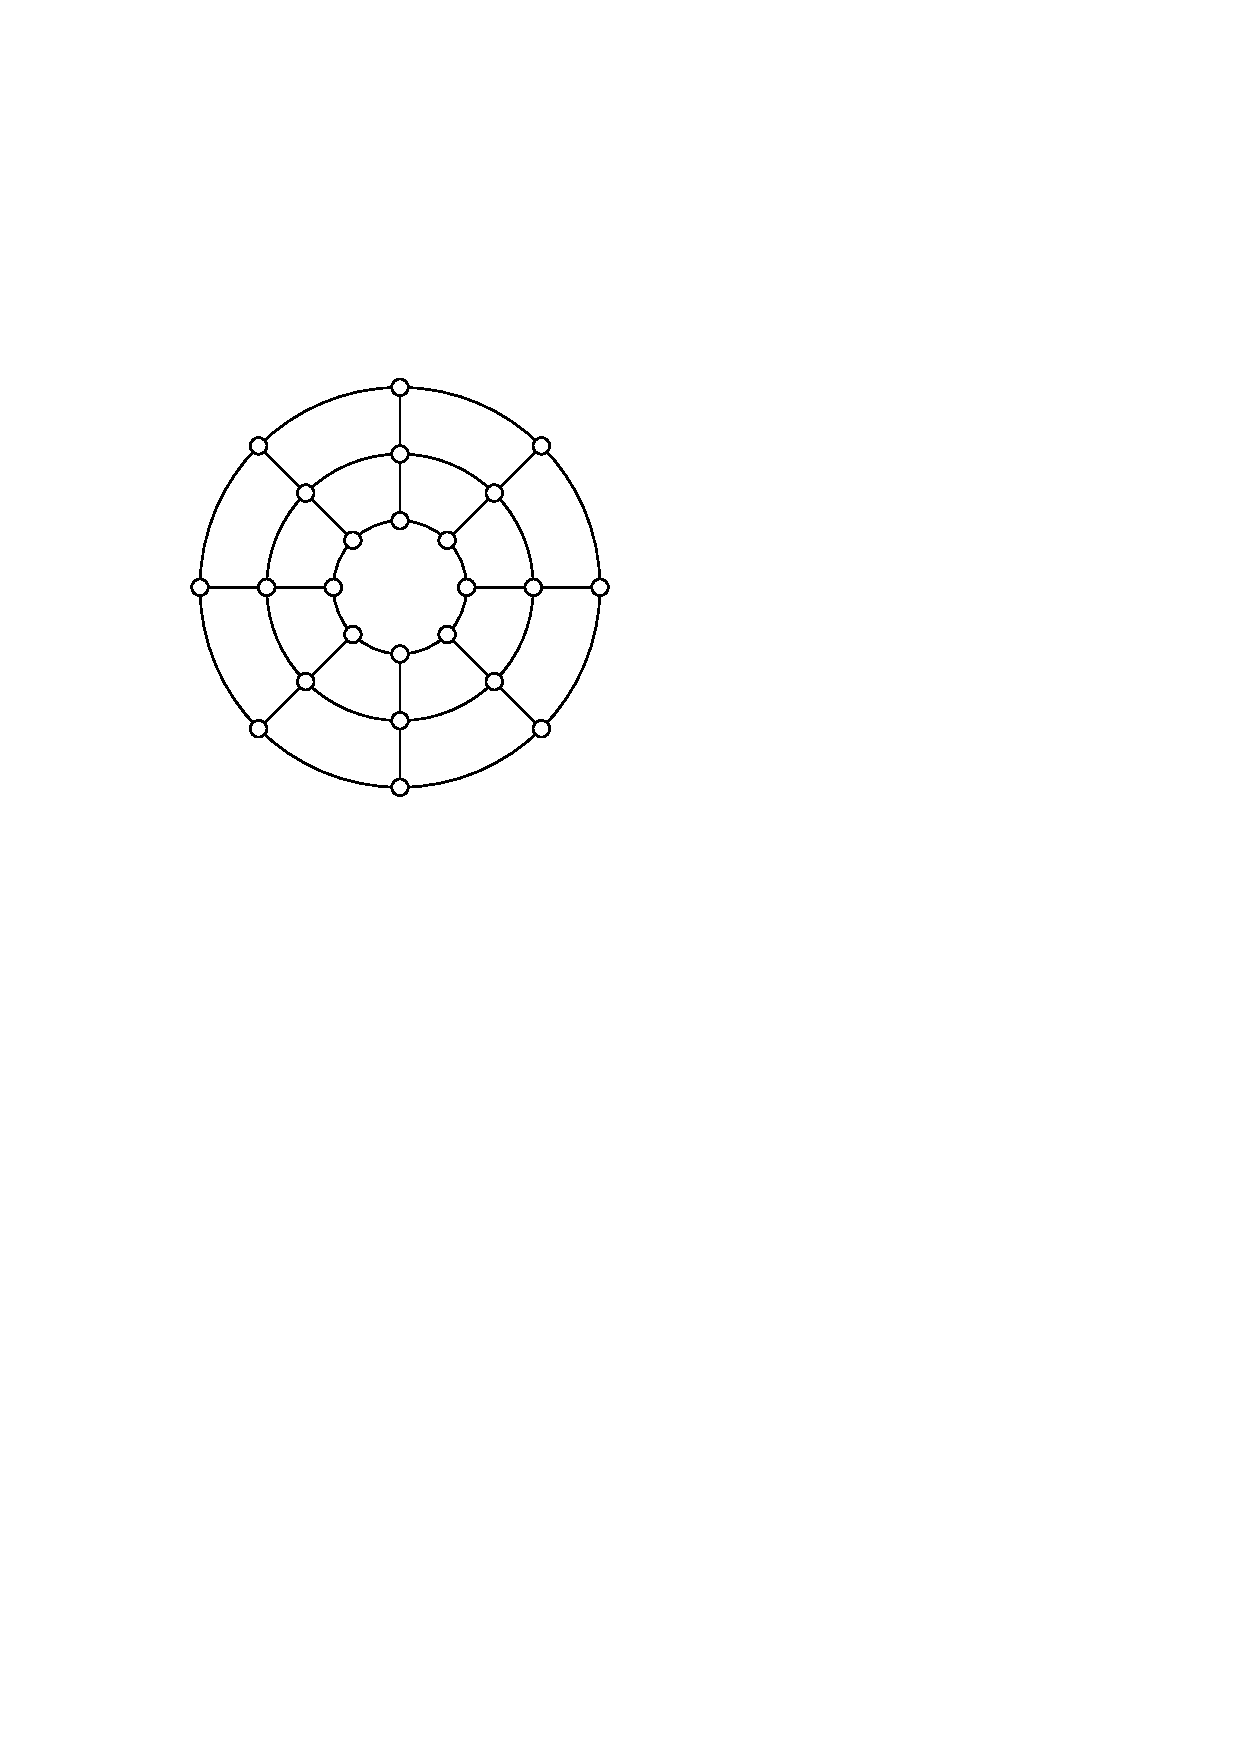
\includegraphics[width=0.23\textwidth]{figures2/ortho.pdf}
	\hfill
	\includegraphics[width=0.23\textwidth,page=2]{figures2/ortho.pdf}
	\caption{Two kinds of ortho-radial grid graphs. Left: Ortho-radial grid graph with $b = 8$ and a central node. Right: Ortho-radial grid graph where $b$ is doubled each time the radius doubles.}
	\label{FIG:orthoradgrid}
	\vspace{-.65cm}
\end{figure}

\bibliographystyle{ACM-Reference-Format}
\bibliography{pfaedle}
\end{document}
